% Official Springer Nature journal template, version 3.1, December 2024.
% One-column working manuscript; numerical references.
% Review revision based on cab6312716321282b1c600b85abebe789085f654.
% Author review before submission: confirm the final interpretation and
% disclose AI-assisted revision in accordance with the applicable journal policy.
\documentclass[pdflatex,sn-mathphys-num]{sn-jnl}
\usepackage{graphicx}
\usepackage{xcolor}
% The class ships \orcidlogo as a bare 
\includegraphics{Orcidlogo.eps}; the
% logo is not distributed with the class, so a local copy is provided and
% scaled/raised to sit with the author names.
\renewcommand{\orcidlogo}{\raisebox{0.7pt}{
\includegraphics[height=7.2pt]{Orcidlogo.eps}}}
\hypersetup{hidelinks,bookmarksdepth=2}
% The bibliography style emits \burl for online references.
\let\burl\url
\usepackage{amsmath,amssymb}
\usepackage{array}
\usepackage{booktabs}
\usepackage{makecell}
\usepackage{needspace}
\usepackage{etoolbox}
% Keep headings with a useful amount of following text; avoid isolated lines.
\let\unpatchedsection\section
\pretocmd{\section}{\Needspace{6\baselineskip}}{}{}
\pretocmd{\subsection}{\Needspace{7\baselineskip}}{}{}
\pretocmd{\subsubsection}{\Needspace{6\baselineskip}}{}{}
\pretocmd{\paragraph}{\Needspace{3\baselineskip}}{}{}
\clubpenalty=10000
\widowpenalty=10000
\displaywidowpenalty=10000
\newcommand{\code}[1]{{\def\{{\textnormal{\textbraceleft}}\def\}{\textnormal{\textbraceright}}\texttt{#1}}}
\raggedbottom
\begin{document}
\title[Correctness Boundaries of Typed Fleet Plans]{Correctness Boundaries of Typed Plans for Natural-Language Robot Fleet Control}
\author*[1]{\fnm{Artem}\sur{Tuzov}\hspace{2pt}\orcid{https://orcid.org/0009-0007-5252-1886}}\email{a.tuzov@innopolis.university}
\author[1]{\fnm{Dmitrii}\sur{Vizitei}\hspace{2pt}\orcid{https://orcid.org/0009-0006-6275-0589}}\email{d.vizitei@innopolis.university}
\author[1]{\fnm{Evgenii}\sur{Shlomov}\hspace{2pt}\orcid{https://orcid.org/0009-0005-8864-5819}}\email{e.shlomov@innopolis.university}
\author[1]{\fnm{Senya}\sur{Belykh}}
\author[1]{\fnm{Anastasia}\sur{Malakhova}}\email{a.malakhova@innopolis.university}
\author[1]{\fnm{Alexander}\sur{Maloletov}\hspace{2pt}\orcid{https://orcid.org/0000-0002-7312-2944}}\email{a.maloletov@innopolis.ru}
\affil[1]{\orgname{Innopolis University}, \orgaddress{\city{Innopolis}, \country{Russia}}}

\abstract{A robot fleet can accept a plan whose assignments, routes, or
completion reports still fail to meet the mission requirements. We examine
these distinctions in a three-level Robot Operating System 2 implementation
with twenty simulated robots. An offline benchmark of 44 cases measures
whether generated plans pass checks on representation and selected
case-specific requirements. Across five local configurations without
constrained decoding, 70.0--87.3\% of responses pass. In the selected
18-run simulation series, every run satisfies its pose-based task conditions.
The series includes two successful repeats that replaced two incomplete
runs after a software change. Separate execution traces document a robot
routed to a pickup already assigned to another carrier, rejection of a
route for a formation whose offsets did not match the requested column,
and an arrival report that omitted a requested robot. A carry task records
ordered zone presence for the same robot. The measured outcome therefore
covers spatial events; physical cargo transfer is outside the evaluation.
The case study identifies which conditions the implemented checks enforce
and which require separate evidence.}

\keywords{Multi-robot systems, Language models, Fleet coordination, Typed plans, Deterministic guards, ROS 2}
\maketitle

\section{Introduction}

Commanding a fleet of mobile robots that share one workspace is a
long-standing problem, and the classical decomposition separates fleet-level
decisions --- which robot goes where, in what order --- from robot-level
execution. Large language models make a natural-language front-end to that
decomposition newly attractive~\citep{saycan,codeaspolicies}: a
model can reason over compact semantic primitives instead of producing control
commands.

\begin{figure}[!htbp]
\centering
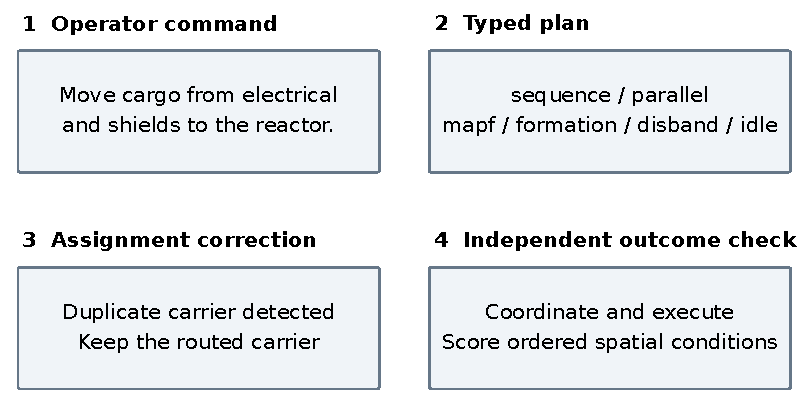
\includegraphics[width=\textwidth]{fig_hero.pdf}
\caption{Illustrative duplicate-carrier correction at the language--coordination
boundary. An additional robot is routed to the same pickup. The guard retains the
robot with the drop-off leg and removes the extra pickup assignment}

\label{fig:hero}
\end{figure}


The difficulty is that a well-formed language response need not describe an
executable fleet action. It may refer to unavailable robots, assign conflicting
goals, or request a formation whose geometry is incompatible with a corridor.
Direct generation of multi-agent path finding (MAPF) solutions by a language
model has failed on tested room and maze instances~\citep{mapfllmfail}. We therefore separate task interpretation from spatial
planning and ask which errors can be handled at their interface.


Hierarchical control, formal intermediate representations, and deterministic
validation are established approaches. Our contribution is a case study of
their coverage in a mobile fleet. We describe the checks at the interfaces
and document execution cases in which a structurally accepted plan still
exhibits an assignment error, a route rejection, or a mismatch between a
component report and the original request.

Research question 1 (RQ1) asks which checks on generated fleet plans fail
under the tested model and serving configurations. To understand
what happens after generation, RQ2 asks which observed assignment and spatial
conflicts the implemented guards handle and which they leave unchecked.
Finally, RQ3 asks why a component can report successful execution without
fulfilling the mission's task-evaluator conditions.

We distinguish plan representation, intended task meaning, spatial
executability, and evaluator completion. The sources behind these claims have
different denominators and provenance; they are not independent replications
of one guard-effect experiment. Figure~\ref{fig:hero} shows a
duplicate-carrier correction; the shared-drop-off comparison is a separate
case (Sec.~\ref{sec:absorb}).

% =========================================================================
\section{Related Work}

An instruction to a robot fleet leaves two different problems to solve:
deciding what the robots should do and finding motions that realize those
decisions. Classical multi-agent path finding addresses the latter once
starts, goals and movement rules have been specified. Conflict-Based
Search~\citep{cbs} resolves path conflicts through constraints, while
Priority-Based Search (PBS)~\citep{pbs} and large-neighborhood repair
(MAPF-LNS2)~\citep{lns2}
offer alternative ways to coordinate paths. The resulting paths
coordinate motion under the specified rules, but do not determine whether
the supplied assignments and goals express a
user's request. A language interface must establish that connection before
path planning can serve the intended task. 
Whether a language model can supply those assignments is a separate
question. PlanBench documents plan-generation failures on its tested models
and tasks~\citep{planbench}.

Grounding language in executable skills is therefore central to early
robot planners based on large language models (LLMs). SayCan~\citep{saycan} combines a language model's
estimate of a skill's usefulness with an affordance estimate of whether the
robot can execute it in the current state. This connects task interpretation
to available behavior without asking the language model to generate motor
commands. Code as Policies~\citep{codeaspolicies} gives the model a more
expressive interface: it composes perception and control APIs into programs,
including control flow and numerical operations. For fleet control the
distinction matters: choosing an available action and assembling a coherent
mission require different checks.

Execution can depart from a plan even when its actions are available. Inner
Monologue~\citep{innermono} feeds observations and success reports back into
language reasoning, allowing subsequent decisions to account for execution.
ProgPrompt~\citep{progprompt} incorporates this concern into program-like
plans through assertions and recovery steps. In its simulated evaluation,
assertions are assessed by an LLM using environment-state information,
whereas our runtime guards apply explicit predicates. Both
approaches make feedback part of planning, and both raise the question our
implementation turns on: what does a reported success establish?

For a robot team, grounding individual actions must be combined with
allocation and coordination~\citep{mrssurvey}.
The task-allocation taxonomy distinguishes single- and multi-task robots,
single- and multi-robot tasks, and instantaneous and time-extended
assignment~\citep{mrta}. Our duplicate-carrier case concerns the assignment
of a single-robot task. SMART-LLM~\citep{smartllm}
uses prompted task decomposition, coalition formation and allocation to
construct a team plan. This makes robot selection part of language-level
planning rather than an input assumed to be correct. RoCo~\citep{roco}
instead uses dialogue between robot-specific language agents to develop a
joint plan, which is checked before a centralized multi-arm planner
generates motion. These designs place coordination at different points in the
pipeline, but both need a connection between the proposed team behavior and
its executor's capabilities; our duplicate-carrier and shared-destination
cases examine that connection.


Formal planning makes constraints explicit. LaMMA-P~\citep{lammap} uses the
Planning Domain Definition Language (PDDL) and heuristic search for
heterogeneous teams. HiP-CL~\citep{hipcl} translates instructions into a
controlled language and then constructs a planning problem with spatial and
resource constraints. LLM+P~\citep{llmp} translates a problem into PDDL and
delegates search to a classical planner. LLM-Modulo~\citep{llmmodulo}
describes a broader pattern in which external verifiers evaluate proposals
and provide feedback. Our checks cover a subset of the properties at that
boundary. Temporal-logic mission planning can synthesize a controller with
guarantees relative to a realizable specification and modeled environment
assumptions~\citep{ltlmission}.

CommandSwarm~\citep{commandswarm} checks generated behavior trees against
allowed swarm primitives. Sangchai et al.~\citep{symbolicwrappers} use
structured tools or PDDL and let a person review the intermediate plan.
Khatana et al.~\citep{verifiermediated} separately ground candidate multi-robot
plans into trajectories and predict inter-robot conflicts to guide
replanning. Their geometric verifier checks trajectory conflicts. Our
case study follows the mobile-fleet interface through assignment and goal
rewrites, a static route rejection, and the evidence used to count mission
completion.

Our study follows these architectural choices through execution in one
implemented fleet. We examine which malformed plans are rejected, which
assignments or destinations are rewritten, and which failures remain after
those checks. The formation case shows how an accepted plan can still fail
because of route geometry, while the completion cases distinguish component
reports from the mission evaluator's ordered spatial conditions. This
analysis characterizes the coverage and limits of the implemented checks.
It does not compare our system's reliability with that of the approaches
reviewed above.

% =========================================================================
\section{System Overview}
\label{sec:overview}





Figure~\ref{fig:arch} shows the operator-chat path. Level~1 turns a natural
language command into a typed plan and applies interface checks. Level~2
coordinates the resulting fleet actions. Level~3 tracks the scheduled
waypoints and executes the control commands.

\begin{figure}[!htbp]
\centering
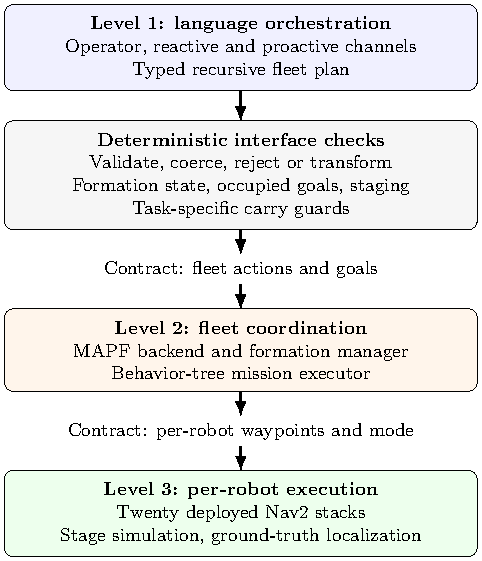
\includegraphics[width=0.64\textwidth]{architecture.pdf}
\caption{Operator-chat path from a typed fleet plan through interface checks,
fleet coordination, and per-robot execution}
\label{fig:arch}
\end{figure}

The interface exposes four distinct correctness questions. Structural
validity concerns admissible node types and fields. Task meaning concerns
the assignments and goals implied by the operator's command. Geometric
feasibility concerns whether robots or formations can traverse the required
space. Evaluator completion concerns whether the specified pose-based events
occur. No implication between these properties follows from the typed
representation alone. Table~\ref{tab:coverage} describes the implemented
coverage and its limits; it is not a formal verification of system safety.


\begin{table}[!htbp]
\caption{Implemented checks and their observed scope}
\label{tab:coverage}
\centering
\setlength{\tabcolsep}{4pt}
\begin{tabular}{>{\raggedright\arraybackslash}p{0.21\textwidth}
                >{\raggedright\arraybackslash}p{0.33\textwidth}
                >{\raggedright\arraybackslash}p{0.34\textwidth}}
\toprule
Property & Check in this implementation & Evidence and limit \\
\midrule
Plan representation & Recursive node and field checks, with selected type coercions
 & E1 also checks case-specific requirements. Acceptance leaves other mission properties open. \\
Robot assignments & Active-formation membership and single-carrier rules
 & Single-carrier rule fired in two selected M2 runs. \\
Occupied goals & Chat-level goal adjustment and planner-level blocked-cell substitution
 & No chat rewrites in the 13 selected language runs. Both mechanisms appear in the additional M4 records. \\
Shared drop-off & Spread coincident goals for distinct carry tasks
 & Logged in three M3 runs. The design does not isolate its effect. \\
Formation assembly & Stage followers and check pose tolerances
 & M4 includes an assembled formation and a separate staging failure. \\
Formation route & Static path check with the planner's footprint approximation
 & M4 rejected a route at planning time. No pre-assembly check of the full oriented formation route. \\
Task completion & Pose samples in specified zones at 5\,Hz, with pickup before drop-off
 & All 18 selected M2/M3 runs satisfy this evaluator. Physical transport and intent are outside the metric. \\
Repair and supervision & Execution remediation, verification repair and bounded mission supervision
 & One supervision pass per selected language run. No remediation or verification-repair attempts in that series. \\
\bottomrule
\end{tabular}
\end{table}


\paragraph{Simulation environment}
Twenty differential-drive robots operate in Stage~\citep{stage} on the
\code{amongus} map ($66.6 \times 37.75$\,m, Fig.~\ref{fig:map}). The world
file places five groups of four around their respective home locations.
The number deployed is distinct from the number moving in any interval.

% =========================================================================
\section{Level 1: Language Orchestration}
\label{sec:orch}

\paragraph{Plan grammar}
In the operator-chat channel, a response contains a natural-language reply
and a plan tree in a JavaScript Object Notation (JSON) object. Four leaf types cover fleet actions --- \code{mapf} (move a robot set to
a goal set), \code{formation} (assemble and hold), \code{disband}, and
\code{idle} (do nothing, with a reason, also the escalation channel) --- and
two containers, \code{sequence} and \code{parallel}, nest recursively. The
following example shows the plan subtree:

\begin{center}\small
\begin{minipage}{\columnwidth}
\begin{verbatim}
{"type":"sequence","steps":[
 {"type":"mapf","robot_ids":[8,9,10,11],
  "goals":[[-8.7,-5.9],[-9.6,-5.9],
           [-8.7,-6.8],[-9.6,-6.8]]},
 {"type":"formation","formation_id":"column_8",
  "leader_ns":"robot_8",
  "follower_ns":["robot_9",
   "robot_10","robot_11"],
  "offsets_x":[-1.5,-3.0,-4.5],
  "offsets_y":[0,0,0]}]}
\end{verbatim}
\end{minipage}
\end{center}

The finite set of node types supports recursive validation and a JSON schema.
These checks cover the implemented structural rules, not arbitrary task semantics or geometric feasibility.


\paragraph{Three channels and grounding}
The reactive channel returns a wait, abort, or replan decision to a
behavior-tree node on warning or error. The proactive observer can send a
flat mode command to the behavior tree. The operator-chat channel uses the
recursive plan grammar and the guards described here. E1 exercises offline
generation for that grammar, and the language runs in E2 use the
operator-chat path. That path can query live pose and task state and compute
room placements through eight allowlisted tools.

\paragraph{Generation and runtime checks}
E1 compares text generation with and without a response schema. Both modes
parse the returned plan and apply case validators. The E2 operator chat
instead enables a tool-calling loop. Enabling that loop allows an auxiliary
tool call but does not require one. In both settings the plan is returned
as JSON.

The operator-chat path validates node types and fields, coerces selected
values, guards active-formation membership, adjusts occupied goals, and
stages robots before assembly. The single-carrier rule removes a redundant
pickup assignment when it can identify the robot routed onward to the
drop-off. The shared-drop-off rule spreads coincident destinations in
eligible cases. Both transformations can change the action requested of a
robot. The pose-based evaluator checks the original task zones after execution.

\paragraph{Execution feedback}
The operator-chat implementation distinguishes three mechanisms: remediation
after an execution error, repair informed by a post-execution state check,
and mission supervision that can request additional work within configured
limits. State verification reads robot poses and formation status. The
results report which mechanisms were invoked in the selected runs.

% =========================================================================
\section{Level 2: Fleet Coordination}


\paragraph{MAPF backends}
The PBS and LNS2 implementations accept robot identifiers and a goal for
each robot through the same action interface. They publish scheduled
waypoints to the robots. The simulation runs reported here use LNS2, which
checks static reachability with its footprint model before planning.

\paragraph{Supporting components}
A formation specification names a leader, followers and per-follower
offsets in the leader's frame. The coordination layer excludes active
followers from independent MAPF assignment and represents the group through
the leader's enlarged planning footprint. This approximation is distinct
from planning with the full, orientation-dependent group shape.
BehaviorTree.CPP~\citep{btcpp} runs the mission tree.


\paragraph{Operational meaning of task completion}
The evaluator samples robot positions at 5\,Hz. A visit task completes
when a robot is observed within 1.5\,m of its target. For a carry task, the
first robot detected in the pickup zone becomes the evaluator's carrier.
The same robot must subsequently be detected in the drop-off zone. One
sample inside each zone is sufficient. This procedure can count a robot
that passes through without stopping, and the recorded carrier may differ
from the one named in the plan.

Pickup and drop-off are logical states. The evaluator checks neither
physical load handling nor the full meaning of the operator's command.
It continues to use the original zones if a guard rewrites a waypoint.
A rewritten goal can therefore receive the same evaluator score while
requiring different motion.

% =========================================================================
\section{Level 3: Per-Robot Execution}
\label{sec:lvl3}

Each robot runs a Robot Operating System 2 (ROS~2) Humble~\citep{ros2}
Nav2~\citep{nav2} stack with namespace substitution and staggered
bring-up. The development record reports discovery and launch difficulties
when starting twenty stacks simultaneously. Stage 2D was selected after
Gazebo Harmonic did not provide a usable real-time factor in the development
setup. These are engineering observations, not controlled simulator or DDS
comparisons.

Localization uses simulator-derived poses. Adaptive Monte Carlo
localization (AMCL) is disabled. During
development, scans from nearby robots caused difficulties with static-map
localization; this motivated removing localization uncertainty from the
case study. The experiments therefore do not test peer-aware localization
or robustness to pose noise. A tuned CycloneDDS profile and a dynamic-blocker
costmap plugin are part of the implementation, but their individual effects
are not measured here.

% =========================================================================
\section{Experimental Design}
\label{sec:design}

We report two complementary evaluations of the implemented system.
The offline benchmark characterizes generated plans; the simulation campaign
examines selected execution outcomes. Neither is a component-removal ablation.


\paragraph{E1 --- offline plan validation}
The benchmark has 44 cases in twelve categories covering navigation,
parallel and sequential composition, formation, disbanding, idle,
escalation and edge cases. Each reported model and decoding condition
contains five scored attempts per case at temperature 0.1. The parser
extracts the plan and applies structural checks. Case validators then
test selected requirements such as robot identifiers, proximity to a
specified destination, and step ordering. A pass means that the response
satisfies those checks. No robots are run in E1.

Schema-off requests use unconstrained text generation and parse a JSON
plan from the result. Schema-on requests pass the plan schema as the
response format. Neither offline condition submits tool definitions.
The local sweep used Ollama, a 16\,GB RTX~5060~Ti, a 32{,}768-token context,
and a 2{,}048-token output limit. The local manifest records partial CPU
offload for Mistral Small 3.2. Hosted runs used OpenRouter with an
8{,}192-token output limit. These are comparisons of the logged
configurations, which differ in model, serving stack, and sometimes
provider or token budget.

Hosted transport errors were handled by rerunning all five attempts of the
affected case and replacing that case's original records. The raw records
log replacements for 18 schema-off and 44 schema-on Nemotron cases, nine
cases in each 397B condition, and 17 schema-on hosted 9B cases. These cells
can mix provider routes. Thus 220 is the number of scored records per cell.
The harness, its prompt builders, per-case prompts, responses, and scoring
scripts support reanalysis of the saved outputs. Exact model snapshots and
complete per-request serving configurations are unavailable.

\paragraph{E2 --- task-evaluator completion in simulation}
M2 consists of four visit tasks and one carry task. M3 consists of six visit
tasks and three carry tasks, two of which share a drop-off location
(Fig.~\ref{fig:map}). The selected descriptive series contains five scripted
M2 runs with fixed assignments, five M2 runs using hosted Qwen3.5-9B, five
M2 runs using hosted Qwen3.5-397B-A17B (cell B), and three M3 runs using the
397B model (cell B-M3). The scripted driver uses the same coordination and
execution layers. Model, routing, allocation and software version vary
across the reported cells.

Selection depended on outcome in B/M2. The
\href{https://github.com/Innopolis-Robotics-Society/llm_swarm/blob/cab6312716321282b1c600b85abebe789085f654/paper/results/e2_mission_series/README_code_versions.md#L15-L64}{development record}
reports
that three original runs completed all five tasks, while runs
\code{20260818\_085836} and \code{20260818\_090145} each stalled at 4/5.
After the single-carrier guard was introduced, those two runs were
replaced by \code{20260818\_093216} and \code{20260818\_093704}. The selected
B/M2 cell thus combines three original successes and two successful
repeats. The bags of the two superseded runs are absent from the public
archive, so their scores are taken from the run history. The 18-run
analysis estimates neither a campaign-wide completion rate nor a guard
effect.

\begin{table}[!htbp]
\caption{Provenance and analysis populations for the simulation evidence}
\label{tab:provenance}
\centering
\setlength{\tabcolsep}{4pt}
\begin{tabular}{>{\raggedright\arraybackslash}p{0.20\textwidth}
                >{\raggedright\arraybackslash}p{0.14\textwidth}
                >{\raggedright\arraybackslash}p{0.54\textwidth}}
\toprule
Series & Runs & Inclusion and evidence \\
\midrule
Selected M2/M3 & 18 & Four cells. Session IDs and base commits are
 recorded. All 18 worktrees were dirty. Thirteen runs have a language
 journal, of which eight have per-phase checkpoints. \\
Superseded B/M2 & 2 & Two runs at 4/5 tasks replaced after a software change.
 The three original successes remain in the selected cell. \\
M3 before/after & 2 + 3 & Two separate pre-guard runs have bags and logs but
 no decision journal. The three post-guard runs are the B-M3 cell above. \\
M4 formation & 4 recorded attempts & Two retained qualitative cases
 (\code{20260818\_140918}, \code{20260819\_073009}). A pilot
 (\code{20260818\_135527}) stopped early and a 42\,s recording
 (\code{20260819\_072231}) with no motion was discarded. All are outside the selected series. \\
\bottomrule
\end{tabular}
\end{table}

The archived session files and logs identify the included runs. A recorded
base commit does not identify the uncommitted changes present in a run. The
comparison uses the task evaluator recorded in \code{/tasks/state} and
the target task list defined for each mission. In completed runs, makespan is the
simulation-time interval from the first recorded task-state sample to the
first sample at which the last target reaches done.

\begin{figure}[!htbp]
\centering
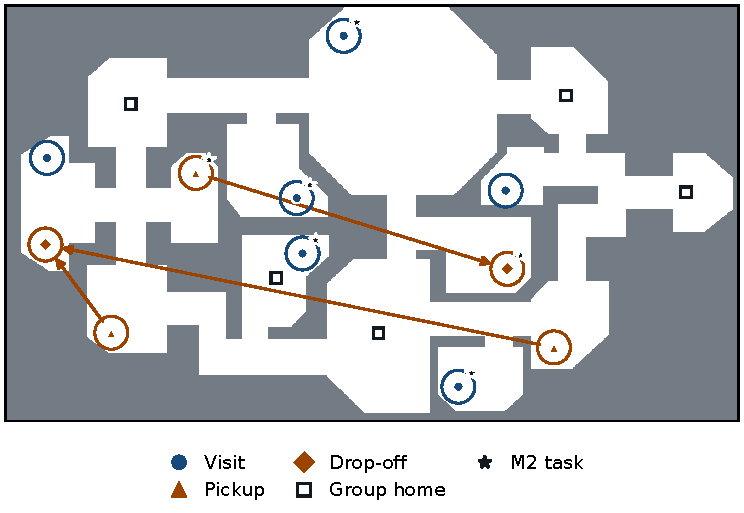
\includegraphics[width=\textwidth]{fig_map.pdf}
\caption{The \code{amongus} map ($66.6 \times 37.75$\,m, 0.05\,m cells) and
the eleven distinct 1.5\,m zones used by the nine M3 tasks. Circles show the
zone boundaries and center markers identify visit, pickup, and drop-off
zones. Arrows link pickup and drop-off locations. Stars mark the M2 subset.
Squares mark the home locations of the five groups of four robots}
\label{fig:map}
\end{figure}

% =========================================================================
\section{Results}
\label{sec:results}

The results are organized around observed boundary failures before the
aggregate scores. Assignment and geometric cases address RQ2; qualitative
completion-report mismatches address RQ3; the offline results characterize
RQ1. Each source retains its own provenance and denominator.

\subsection{Assignment defects and shared-destination conflicts}
\label{sec:absorb}

The inspectable plans reveal an assignment-level defect relevant to RQ2. All
13 language runs retain a plan and a decision journal, but only eight also
retain per-phase checkpoints; the five model-9b runs predate checkpointing and
store a single record, so execution order is inspectable only for the later
cells. Among the 13 generated plans, 5 carry the same assignment defect: the plan
assigns two robots to carry a single item. In three model-9b runs the extra
carrier is visible in the stored plan; in two cell-B runs the single-carrier
guard had already removed it, and the defect is recorded only by the guard
counter. An extra robot sent to the pickup can occupy space needed by the
intended carrier. The count describes this inspected set, not the prevalence
of defects across unseen missions.


\paragraph{Duplicate-carrier assignments}
Three model-9b runs visibly route an extra robot to the pickup and still
complete M2. In the two original incomplete B runs, the development record
attributes the stall to robot~5 reaching the pickup before robot~1, which
was assigned the drop-off leg. The guard later removed an extra pickup
assignment in each of the two replacement runs. Both replacements
completed M2. The guard counters establish the recorded intervention.
The successful uncorrected runs and the outcome-dependent selection limit
what this comparison establishes about completion.


\paragraph{Shared-drop-off execution conflict}
M3 assigns two carry tasks to the same drop-off center
(Fig.~\ref{fig:map}). This conflict follows from the mission specification.
Both archived pre-guard runs (\code{20260815\_153035} and
\code{20260815\_154541}) complete 8/9 tasks. Each of the three B-M3 runs
completes 9/9. In run \code{20260818\_111548} the guard changed the common
target $(-29.65,-2.85)$\,m to $(-28.90,-2.85)$\,m for robot~3 and
$(-30.40,-2.85)$\,m for robot~16. Both goals are 0.75\,m from the specified
center and inside the original evaluator zone. The logs show spreading
in all three post-guard runs. The two series differ in software version
and provider routing, and the pre-guard journals are absent. These records
document the intervention and outcomes without isolating its effect.

\subsection{Case study: an assembled formation with a rejected route}
In the interactive M4 session \code{20260819\_073009}, the operator asked
for a column. The model returned \code{offsets\_x=[0,0,0]} and
\code{offsets\_y=[1.5,-1.5,3.0]}, a line abreast with a 4.5\,m span between
the outer centers. The formation assembled at the generated offsets and
reached stable status after 6.5\,s. The logged fraction of broken samples
was zero. On a subsequent move request, LNS2 reported that there was no
static path for the leader under its enlarged footprint model.

This trace separates three checks. The plan passes structural validation,
the generated offsets disagree with the requested geometry, and the
planner rejects a route under its footprint approximation. The system
does not check an oriented trajectory for the entire formation before
assembly. The log therefore establishes rejection by the implemented
planner for the requested start and goal. In a separate M4 run
(\code{20260818\_140918}), the same column request elicited
\code{offsets\_x=[-1.5,-3.0,-4.5]}. These two cases show variation in the
generated offsets. They provide no estimate of its frequency.


\subsection{Local action reports and mission conditions}
\label{sec:failures}

The M4 run \code{20260818\_140918} exposes a chain of failures during
formation staging. A replan temporarily benched robot~0 and replaced the
requested set with the smaller set of planned robots. The action later
reported \emph{All agents arrived} although robot~0 was still at its
starting position. In a subsequent leg, the planner substituted a free
cell for a blocked goal. The formation manager reported that robot~3
was 1.97\,m from its required slot, outside its 0.50\,m staging tolerance.
The executor learned of the refusal only at the step timeout. These
observations come from one development trace and are not counted as
independent failures.

An arrival report describes the action that the component tracked. The
same report can omit a requested robot or concern a substituted goal.
The case motivates recording the original request, effective action and
completion condition separately.

\subsection{Offline plan validation results}
\label{sec:planacc}

Table~\ref{tab:e1} gives the E1 scores. In the local schema-off runs, the
9B configuration has the highest observed call-level rate (192/220). It
leads the 24B and 14B configurations by 8.6 and 12.3 percentage points,
respectively, calculated before rounding the displayed rates. Five repeats
measure response variation on the same cases. For example, 154/220
responses pass for the local 4B model, while 41/44 cases have at least one
pass in five tries.

The published scoring script assigns one diagnostic category per failed
response by a fixed priority of error strings. Across the 1{,}100 local
schema-off records, 259 fail. The categories include formation fields or
staging (82), structure (81), goals (34), unparseable JSON (34), escalation
reason (5), robot identifiers (1), and other validator messages (22).
These are script labels: for example, a goal error can concern arity or
the requested destination. For Mistral Small 3.2, the same offsets-arity
message accounts for 20 of 47 failures, and the most frequent failed
response is byte-identical across eight records. This is evidence of a
recurring error, not of deterministic generation.

\begin{table}[!htbp]
\centering
\caption{Offline validation on 44 cases with five scored responses per case
and condition. Call rate is the percentage of 220 responses that passed.
Case rate is the percentage of 44 cases with at least one pass in five
attempts. Model sizes are nominal; for mixture-of-experts models they are
total/active parameters. n/d denotes an undisclosed size. A dash denotes an
unreported condition}
\label{tab:e1}
\setlength{\tabcolsep}{3.2pt}
\begin{tabular}{lccccc}
\toprule
& & \multicolumn{2}{c}{Schema off} & \multicolumn{2}{c}{Schema on} \\
\cmidrule(lr){3-4}\cmidrule(lr){5-6}
Model & Size & Call (\%) & Case (\%) & Call (\%) & Case (\%) \\
\midrule
\multicolumn{6}{l}{\emph{Local}}\\
Qwen3.5-4B & 4B & 70.0 & 93.2 & 77.7 & 95.5 \\
Gemma 3 12B & 12B & 71.4 & 72.7 & --- & --- \\
Qwen2.5-14B & 14B & 75.0 & 81.8 & 75.5 & 81.8 \\
Qwen3.5-9B & 9B & 87.3 & 95.5 & 19.1 & 22.7 \\
Mistral Small 3.2 & 24B & 78.6 & 81.8 & --- & --- \\
\midrule
\multicolumn{6}{l}{\emph{Hosted}}\\
Qwen3.5-9B & 9B & 90.5 & 97.7 & 51.4 & 61.4 \\
Gemini 2.5 Flash & n/d & 89.5 & 90.9 & 80.9 & 86.4 \\
Nemotron 3 Ultra & 550B/55B & 90.5 & 97.7 & 88.6 & 95.5 \\
Qwen3.5-397B-A17B & 397B/17B & 93.2 & 100.0 & 95.0 & 100.0 \\
\bottomrule
\end{tabular}
\end{table}

\subsubsection{Decoding configurations}
\label{sec:hosted}
Call-level scores under schema constraints rise for the local 4B and 14B
configurations and fall for the local 9B configuration. Hosted differences
also vary in direction. For example, the 397B/17B score rises from 93.2\%
to 95.0\% while Gemini falls from 89.5\% to 80.9\%. In the hosted
comparison, the provider and its support for the response schema can
affect both the output and whether a request succeeds. These observations
describe the tested configurations. They do not identify a general
decoding or model-size effect.

\subsection{Task-evaluator completion in the selected series}
Every included run satisfies all of its target task conditions
(Table~\ref{tab:e2}). In the original B/M2 series, 3/5 runs completed all
tasks according to the run history. The two incomplete runs reached 4/5.
After the two replacements, 5/5 runs in the selected B/M2 cell complete all
tasks. The table reports the selected runs' outcomes and timing.

\begin{table}[!htbp]
\centering
\caption{Selected M2/M3 runs. Task counts are pose-based outcomes per run.
Makespan is the mean and sample standard deviation (SD) in simulation seconds.
Language-loop time is the mean cumulative wall-clock duration recorded in
the decision journals, including any auxiliary calls or retries within the loop}
\label{tab:e2}
\setlength{\tabcolsep}{4pt}
\begin{tabular}{llcccc}
\toprule
Cell & Mission & \makecell{Full\\runs} & \makecell{Tasks\\per run}
 & \makecell{Makespan (s)\\mean $\pm$ SD} & \makecell{Language\\loop (s)} \\
\midrule
no-LLM   & M2 & 5/5 & 5/5 & $203.5 \pm 10.6$ & 0 \\
model-9b & M2 & 5/5 & 5/5 & $252.2 \pm 26.6$ & 9.5 \\
B        & M2 & 5/5 & 5/5 & $260.0 \pm 16.5$ & 31.6 \\
B-M3     & M3 & 3/3 & 9/9 & $587.7 \pm 67.0$ & 51.2 \\
\bottomrule
\end{tabular}
\end{table}

\paragraph{Timing and fleet activity}
The M2 mean makespan ranges from 203.5 to 260.0 simulation seconds.
The mean language-loop duration ranges from 0 to 31.6 wall-clock seconds.
The analysis uses the final cumulative counter for the unique mission
record in each language run.
The intervals have different clocks and start events, and allocation and
software version vary across the cells. We report them separately.
Odometry records show that 9--10 distinct robots per selected run traveled
at least 0.5\,m over the recording. This measures activity over the run,
without estimating peak simultaneous motion.

\paragraph{Observed mechanism use}
None of the 13 selected language runs invoked remediation or verification
repair, and none triggered the active-formation guard or chat-level
occupancy rewrites. Each logged one supervision step. Twelve runs made no
auxiliary calls. One B-M3 run (\code{20260818\_113030}) called
\code{list\_tasks} once and \code{verify\_plan\_execution\_state} twice.
The two additional M4 records contain 10 and 33 auxiliary calls. The
available context differs across missions, and the records do not
establish why the model chose to call a tool.


\section{Discussion}
\label{sec:discussion}

For RQ1, the offline benchmark distinguishes failures to parse a plan from
failures on selected requirements for robot selection, goals, and step
composition. Differences across decoding settings include both gains and
losses. The scored responses describe the tested cases and configurations.
They have no paired mission outcomes for estimating the predictive value of
structural validity.

For RQ2, the carry cases distinguish a redundant pickup assignment from a
shared drop-off requested by the operator. The first can be corrected by
removing a pickup assignment. The second can be addressed by adjusting the
two destinations within the original zone. A formation can also satisfy
the structural and assembly checks while its generated shape differs from
the request and the planner rejects the route. These cases show which
properties require checks beyond the plan representation.

For RQ3, a component can report success for a reduced robot set or
substituted waypoint while the original action remains incomplete. The
evaluator provides separate evidence of the specified spatial events.
The evidence does not establish physical load transfer, collision safety,
or full preservation of intent. The cases motivate logging the original
action, its transformed action, the component report, and the evaluator
outcome as separate records.

\section{Limitations}
\label{sec:limitations}

The study uses one Stage map, simulator-derived poses, two main mission
specifications and a small, selected run series. Five language runs have
only one journal record each. Dirty worktrees prevent exact reconstruction
from the recorded commit IDs, and the superseded B/M2 outcomes come from
the development record. The M3 comparison changes software version and
provider routing. A controlled guard comparison would require fixed
conditions and a prespecified record of all attempts.

E1 repeats 44 case designs. Exact model revisions and complete serving
settings are unavailable, and hosted transport replacements can change the
provider. E2 uses a task-state interval in simulation time and separately
records language-loop duration in wall-clock time. It does not measure
operator-to-completion latency or isolate the cost of language orchestration.

The task metric samples zone presence. It does not measure stopping,
load handling, or independent collision and intent outcomes. No fleet-size
sweep or peak concurrency measurement is available. The observed
formation route rejection applies to the planner's footprint model.
Inactive repair counters and qualitative development observations do not
establish reliability or failure rates.

\section{Conclusion}

This case study documents how structural validity, task meaning, route
feasibility and evaluator completion differ in a typed-plan interface for
robot fleets. Offline validation finds recurring errors in formation
fields, structure and goals. Simulation traces show how assignment guards,
goal transformations and planner checks act on accepted plans, and how
a component's report can omit part of the original request. The results
characterize the implemented checks and the cases in which they were
exercised. They provide specific conditions to test in future controlled
evaluations.

\backmatter

\section*{Statements and Declarations}

\subsection*{Competing Interests}
The authors have no relevant financial or non-financial interests to disclose.

\subsection*{Funding}
\emph{[Funding statement to be confirmed with the project supervisor before
submission. The work was carried out as part of the authors' employment at the
Institute of Robotics and Computer Vision, Innopolis University; whether it
constitutes external funding is for the institution to state.]}

\subsection*{Ethics Approval}
Not applicable. This study did not involve human participants or animals.

\subsection*{Consent to Participate}
Not applicable.

\subsection*{Consent for Publication}
Not applicable.

\subsection*{Use of Generative AI}
OpenAI Codex (0.135.0) and Anthropic Claude Code (2.1.159) were used to write
the implementation code and as assistants in preparing the manuscript,
including the figures. All text, results and interpretations were reviewed by
the authors, who take full responsibility for the content.


\subsection*{Data Availability}
The benchmark outputs, session metadata, logs, derived metrics, and
analysis scripts are in the
\href{https://github.com/Innopolis-Robotics-Society/llm_swarm/tree/cab6312716321282b1c600b85abebe789085f654/paper/results}{results directory at the archived repository revision}.
The recorded bags are available in the
\href{https://drive.google.com/drive/folders/1fpkuhE1f3ET2YIJLI5sV4jPzE1IJophs?usp=sharing}{public results archive},
\code{llm\_swarm\_results\_2026-11-04.tar.zst} (135\,MB).
Its SHA-256 checksum is
\code{3866f1fce6254243\hspace{0pt}986b0052e2fc0d60\hspace{0pt}39eadc351e10c460\hspace{0pt}f4ed0feec69f740d}.
A per-file manifest accompanies the archive. With the archive unpacked,
run the repository's \code{paper/results/scripts/analyze\_sessions.py}
with \code{--sessions} pointing to the unpacked
\code{results/e2\_mission\_series} and \code{--json} to export per-run metrics.
The two superseded B/M2 bags are absent. Their scores and replacement
identifiers are documented in the run history.

\subsection*{Code Availability}
The ROS~2 stack, benchmark harness, and analysis scripts are available at
\href{https://github.com/Innopolis-Robotics-Society/llm_swarm/tree/cab6312716321282b1c600b85abebe789085f654}{repository revision \code{cab6312}}.
This revision records the analysis and documentation. It does not
capture the uncommitted changes in the historical simulation runs.
Licence declarations, where present, are in the individual packages.

\subsection*{Author Contributions}
A.T.: Conceptualization, Methodology, Software, Investigation, Data curation,
Writing---original draft, Writing---review and editing, Project administration.
D.V.: Software, Investigation, Writing---review and editing.
E.S.: Conceptualization, Methodology, Software, Investigation, Supervision,
Project administration, Writing---review and editing.
S.B.: Software, Investigation, Visualization.
A.Mal.: Software, Validation.
A.Malol.: Supervision, Conceptualization, Writing---review and editing.

% =========================================================================

%BRK%
% The bibliography uses its native heading spacing and tighter entry gaps.
\begingroup
\let\section\unpatchedsection
\setlength{\bibsep}{0.5em}
\interlinepenalty=10000
\bibliography{refs}
\endgroup

\end{document}
